\kmuttchapter{THEORETICAL BACKGROUND}

%The electronic properties of conventional material such as silicon

\section{Klein tunneling effect} \label{2sec:klein effect}
    Klein tunneling refers to a relativistic particles penetrate through the potential barrier without backscattering.
    These properties was once unique to the high-energy particles, where it can only be observed in the system with high-driven voltage.
    In 2006, this effect is predicted to occur in low-energy system of graphene \cite{Katsnelson2006a}.
    This is because the electron in graphene mimics the relativistic massless Dirac particle and obey massless Dirac equation
    \begin{align} \label{2eq:Hamiltonian}
        \hat{H} = -i\hbar v_F \sigma \nabla 
    \end{align}
    where $v_F \approx 10^6 \mathrm{ms^{-1}}$ is Fermi velocity, $\sigma = (\sigma_x, \sigma_y)$ is Pauli matrix. 
    \begin{figure}[H]
        \centering
        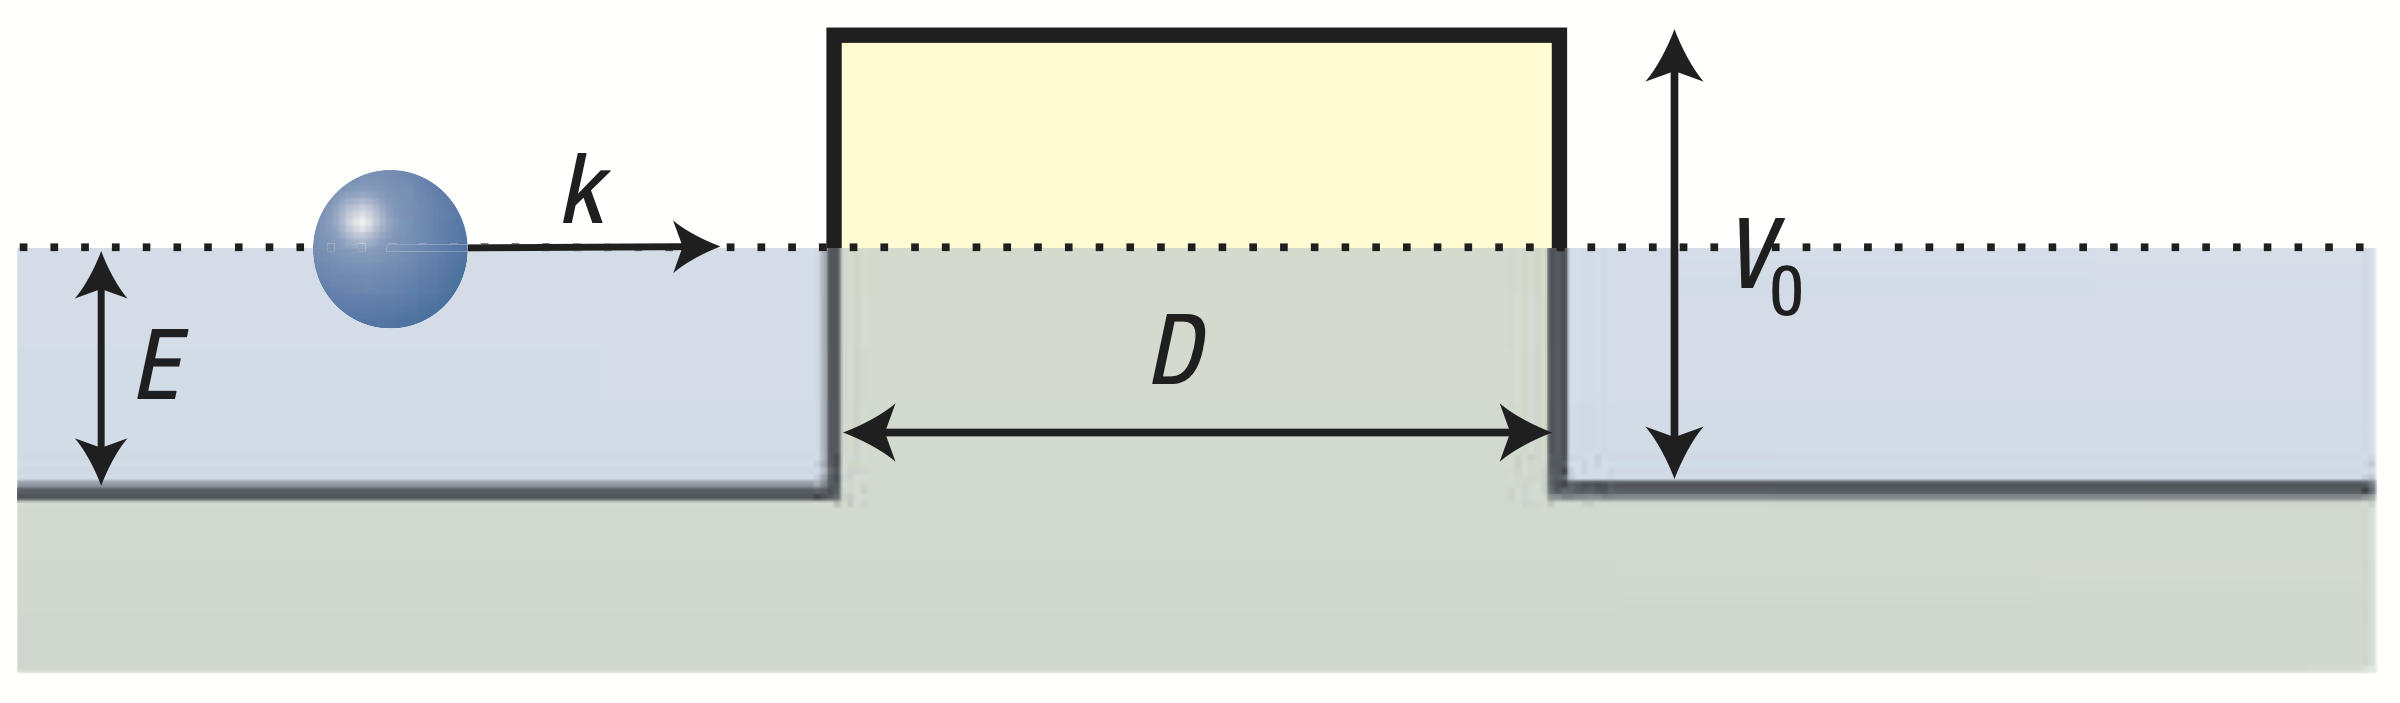
\includegraphics[width=0.7\linewidth]{fig/Chap 2/electron propagation.png}
        \caption{Schematic diagram of electron propagation through the potential barrier of height $V_0$ and width $D$}
        \label{2fig:electron propagation}
    \end{figure}
    The electron propagation can be modeled as in Fig. \ref{2fig:electron propagation}, consisting of three transport region where the Fermi energy of electron is below the potential barrier.
    By solving Eq. \ref{2eq:Hamiltonian}, the wave function of each region can be expressed as follows
    \begin{equation} \label{2eq:wave function}
        \begin{aligned}
            \psi_1 &= \begin{cases} (e^{ik_x x}+re^{-ik_x x})e^{ik_y y}, &x<0,\\
                (ae^{i q_x x}+be^{-i q_x x})e^{ik_y y},  &0<x<D,\\
                te^{ik_x x + ik_y y},  &x>D,
                \end{cases}\\
            \psi_2 &= \begin{cases} s(e^{ik_x x+i \phi}-re^{-ik_x x-i \phi})e^{ik_y y},  &x<0,\\
                s^\prime(ae^{i q_x x+ i \theta}-be^{-i q_x x- i \theta})e^{ik_y y}, &0<x<D,\\
                ste^{ik_x x + ik_y y+ i \phi}, &x>D,
                \end{cases}
        \end{aligned}
    \end{equation}
    where $k_x = k \cos{\phi}$ and $k_y = k \sin{\phi}$ are x- and y-component wavevector outside the barrier region, respectively.
    $q_x = \sqrt{(E-V_0)^2/(\hbar v_F)^2-k_y^2}$ is x-component wavevector inside the barrier region. 
    $s = \mathrm{sgn}(E)$ and $s^{\prime} = \mathrm{sgn}(E-V_0)$. 
    Since the wave function of each region has to be continuous at the boundary, we can substitute $x = 0$ and $x = D$ to Eq. \ref{2eq:wave function}, which give
    \begin{equation} \label{2eq:boundary condition}
        \begin{aligned}
            1+r-a-b&=0\\
            s(e^{i\phi}-e^{-i\phi}r)-s\prime (e^{i\theta}a-e^{-i\theta}b)&=0\\
            e^{iDq_x}a+e^{-iDq_x}b-e^{iDk_x}t&=0\\
            s \prime (e^{iDq_x+i\theta}a-e^{-iDq_x-i\theta} b)-se^{iDk_x+i\phi}t&=0\\
        \end{aligned}
    \end{equation}
    where r and t is the reflection and transmission coefficient, respectively. Which can be obtained by solving the system of equations above.
    The reflection coefficient has the following expression
    \begin{align} \label{2eq:reflection coefficient}
        r=2ie^{i\phi}\sin{(q_xD)}\times\frac{\sin{\phi}-ss^{\prime}\sin{\theta}}{ss^{\prime}[e^{-iq_xD}\cos{(\phi+\theta)}+e^{iq_xD}\cos{(\phi-\theta)}]-2i\sin{(q_xD)}}
    \end{align}
    Since $T = |t|^2 = 1-|r|^2$, the transmission probability can be expressed as follow
    \begin{align} \label{2eq:transmission probability}
        T = \frac{\cos^2{\phi}}{1-\cos^2{q_x D}\sin^2{\phi}}
    \end{align}
    Fig. \ref{2fig:Klein tunneling} shows the polar plot of Eq. \ref{2eq:transmission probability}. 
    At the incident angle $\phi = 0$, electron tunnels through the barrier with probability of one no matter the height of the potential barrier.
    This is the feature unique to massless Dirac fermion called Klein tunneling.
    \begin{figure}[H]
        \centering
        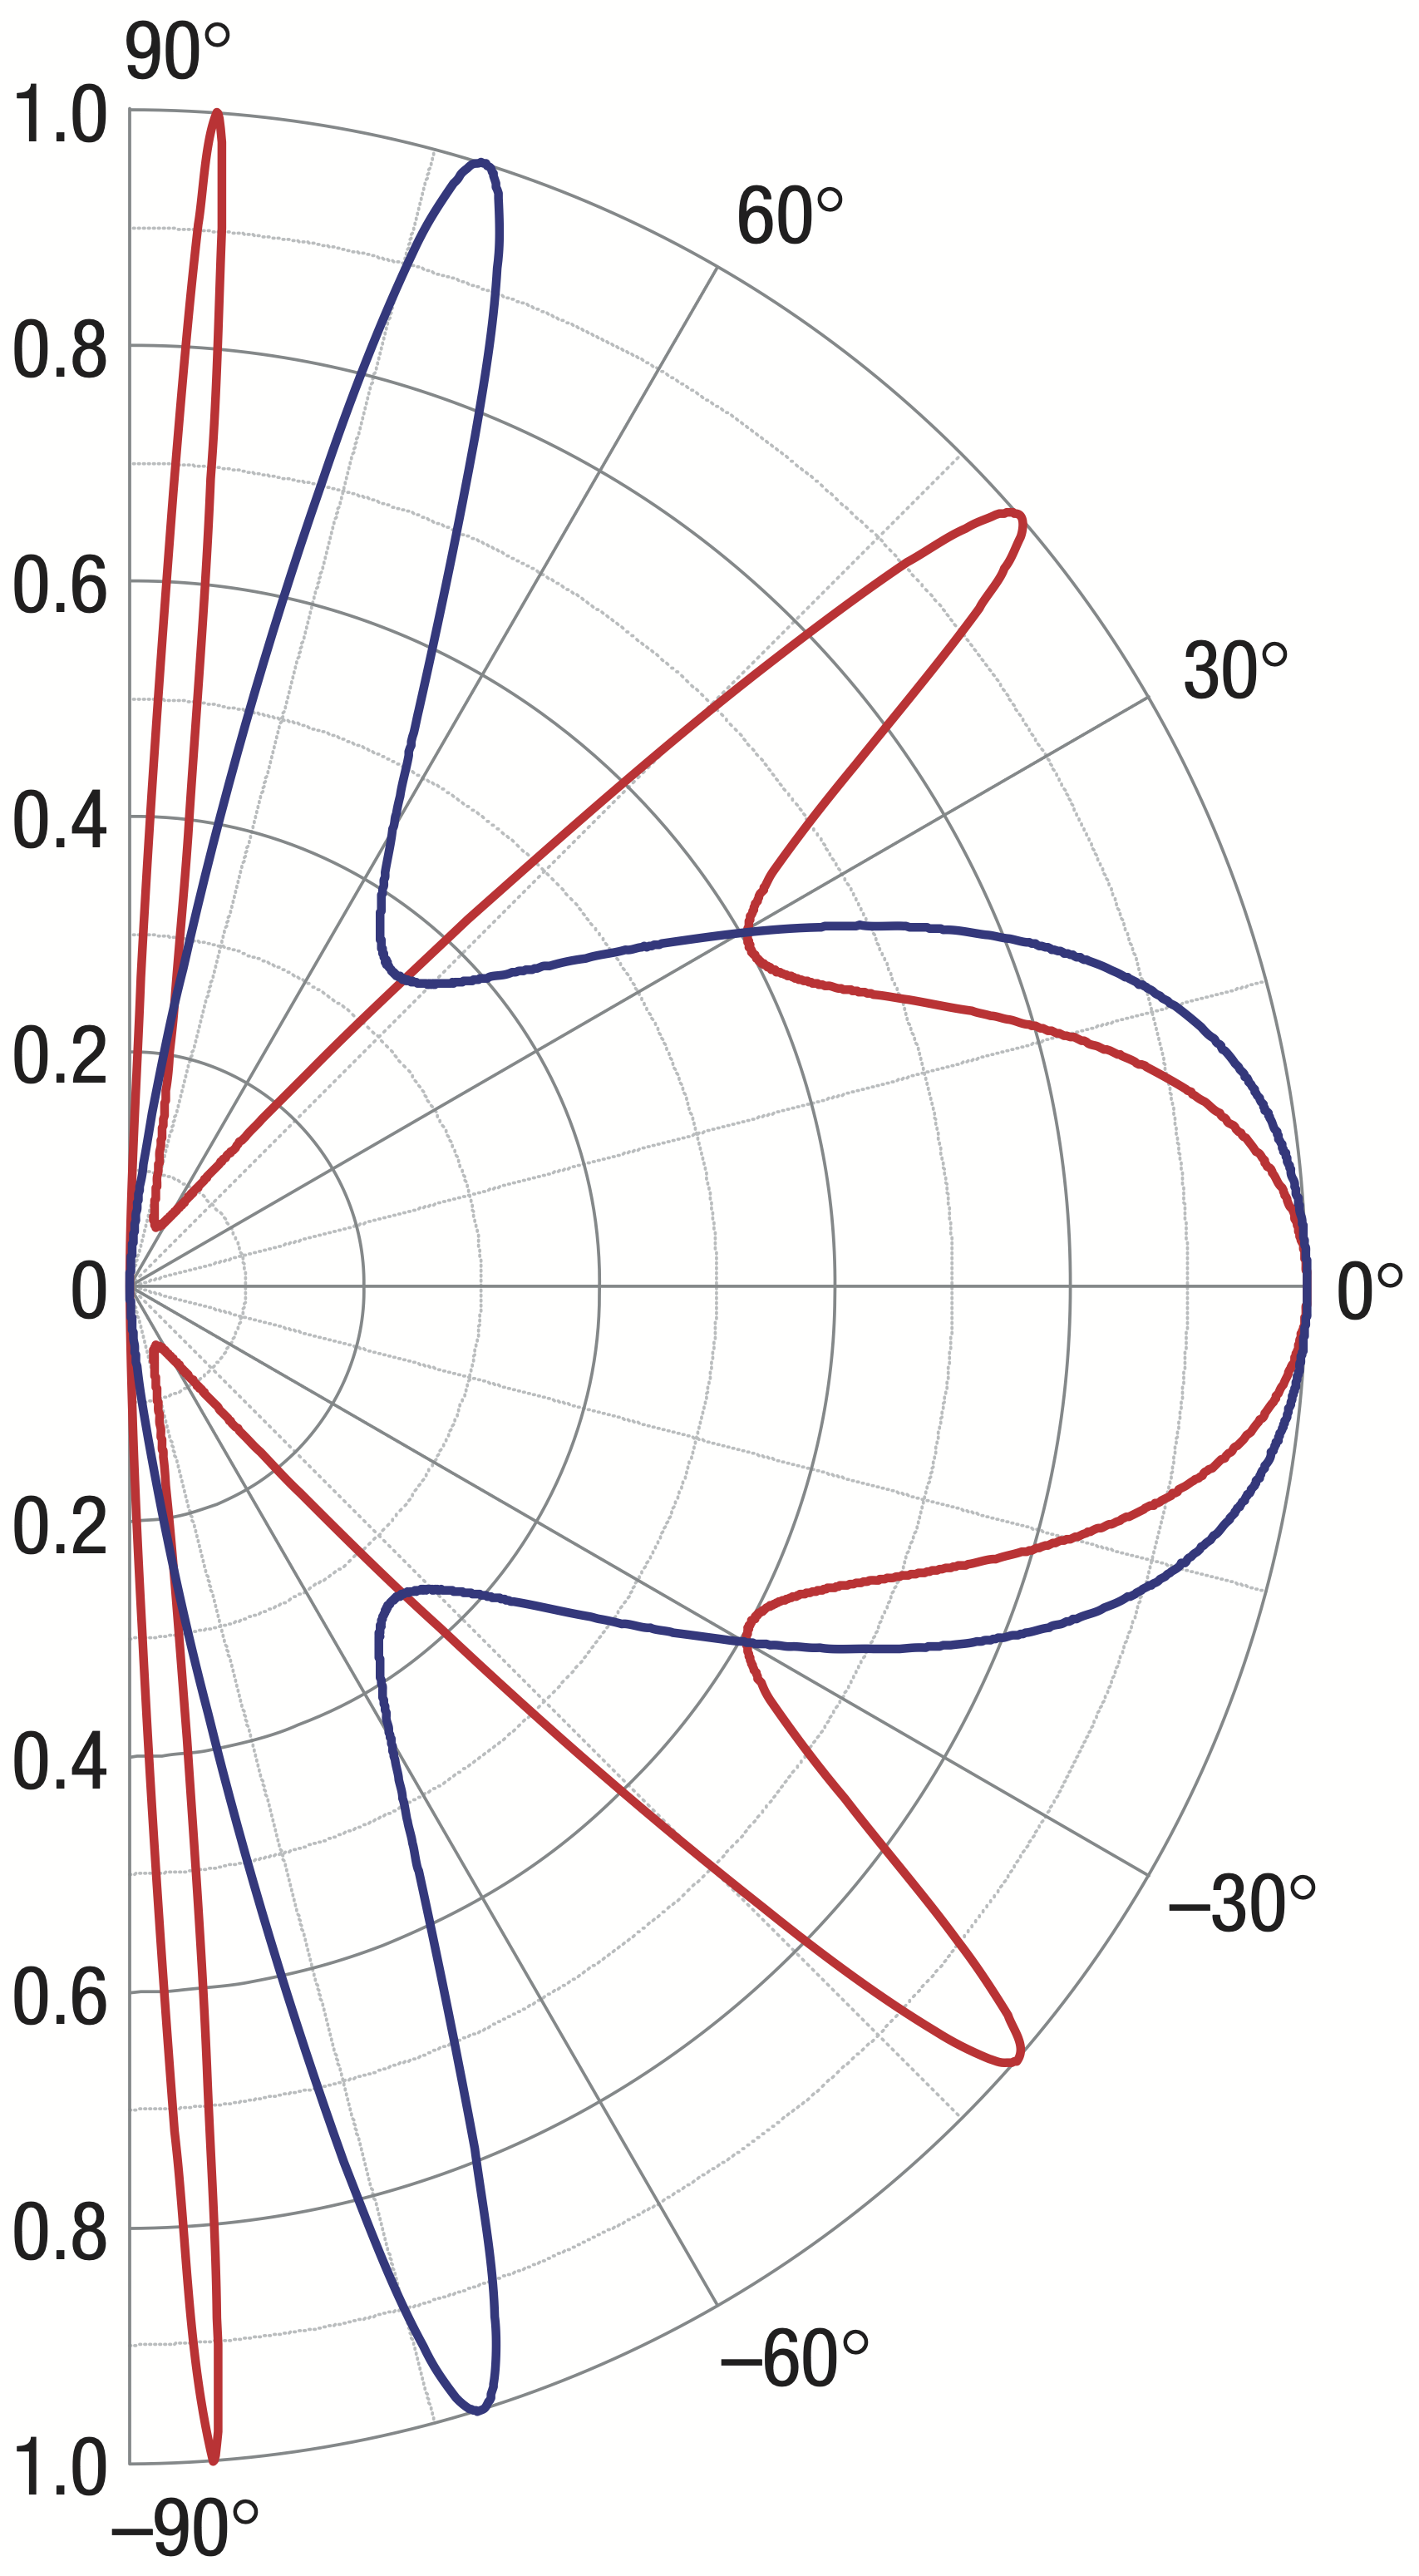
\includegraphics[width = 0.3\linewidth]{fig/Chap 2/klein tunneling.png}
        \caption{The transmission probability as a function of incident angle with different barrier height. 
                    $V_0 = 200$ meV for red curve and $285$ meV for blue curve \cite{Katsnelson2006a}.}
        \label{2fig:Klein tunneling}
    \end{figure}

\section{Electronic transport of electron in graphene under the influence of magnetic field} \label{2sec:transport in B field}

\section{Asymmetric tunneling of electron in tilted Weyl cone systems} \label{2sec:asymmetric tunneling}
    The electronic structure of pristine graphene is often symmetric and non-tilted, 
    which indicate that the transmission of electron is symmetric with respect to normal incident angle as shown in section \ref{2sec:klein effect}.
    Unlike the Dirac cone of graphene, in 3-dimensional Weyl semimetals, the Weyl cone around the Weyl point is generally tilted and anisotropic as Weyl points are not located on high-symmetry k-points.
    A tilted Weyl fermion can be described by the low energy Weyl Hamiltonian with asymmetric velocities
    \begin{align}\label{2eq:Hamiltonian titled}
        H = V_0 + \sum_{i} \hbar k_i(\sigma^{i} v_i + w_i) 
    \end{align}
    where $\sigma^i$ are the Pauli matrices, $v_i$ are the velocities in 3 dimensions, and $V_0$ is the potential barrier height.
    $w_i$ is the tilt of Weyl cone in the unit of velocity. The model of interest is shown in Fig. \ref{2fig:transistor} with the potential profile $V_{(x)} = V_0[\Theta(x)-\Theta(x-L)]$.
    By solving the Hamiltonian above, the components of the wave functions are written as
    \begin{align} \label{2eq: wave functions}
        \psi_{\pm} = \frac{1}{\sqrt{2}}e^{i k^{\rightarrow} r^{\rightarrow}}
        \begin{pmatrix}
            1 \\
            e^{i \phi} \sec{\gamma (\pm 1 + \sin{\gamma})}
        \end{pmatrix}= 
        \begin{pmatrix}
            \psi_a \\
            \psi_b^{\pm}
        \end{pmatrix}   
    \end{align}
    The transmission probability can be calculated by matching both components of the wave functions at the interfaces.
    The wave vector outside the potential barrier is expressed as
    \begin{equation}\label{2eq:outside wavevector}
        \begin{aligned} 
            k_x &= k_F \cos{\gamma} \cos{\phi},\\
            k_y &= k_F\cos{\gamma} \sin{\phi},\\
            k_z &= k_F \sin{\gamma}\\
        \end{aligned}
    \end{equation}
    and wave vector inside the potential barrier is
    \begin{align} \label{2eq:inside wavevector}
        q_x = \frac{\sqrt{(E_F-V_0-\hbar k_y w_y)^2 - \hbar^2 v_F^2 (k_y^2 + k_z^2)}}{\hbar v_F}.
    \end{align}
    The angles of electron propagation inside the potential barrier 
    \begin{equation} \label{2eq:angles}
        \begin{aligned}
            \theta &= \arctan{\left(\frac{k_y}{q_x}\right)},\\
            \alpha &= \arctan{\left(\frac{k_z}{q_x} \cos{\theta}\right)}.\\
        \end{aligned}
    \end{equation}
    can be calculated by considering the conservation of the transverse wave vectors $k_y$ and $k_z$ at the barrier interface $x = 0$. 
    \begin{figure}[H]
        \centering
        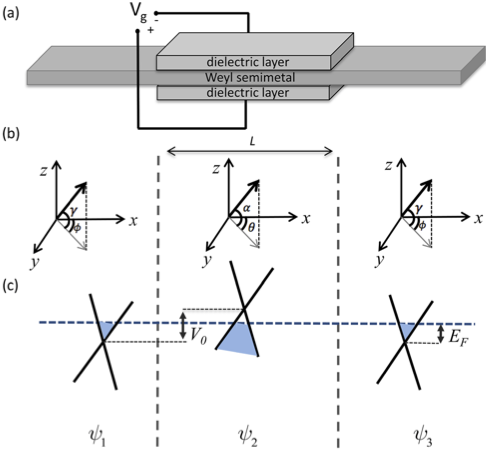
\includegraphics[width = 0.6\linewidth]{fig/Chap 2/2transistor.png}
        \caption{transistor}
        \label{2fig:transistor}
    \end{figure}


    In the case of non-tilted Weyl cone system, the transmission probability is symmetric with respect to $\phi = 0$ and $\gamma = 0$ as shown in Fig. \ref{2fig:anomalous1}.
    Which similar to the transmission of electron in graphene except that it is confined to two dimensions, whereas the Weyl semimetal is three dimensions.
    This symmetric transmission becomes asymmetric when the Weyl cone is tilted along one of the transverse directions as shown in Fig. \ref{2fig:anomalous2}.
    In other word, the transmission is shifted to the direction of the tilt. 
    This can be understood by considering the Fermi surfaces in Fig. \ref{2fig:anomalous fermi surface}.
    In the case of $\phi > \phi_{a,b}$, $q_x$ becomes imaginary and the electron is totally reflected.
    The shaded angles show the allowed range where the electron can propagate through the barrier.
    The analytical form of the critical angle of incident electron is found as
    \begin{equation} \label{2eq:phi a}
        \phi_a = \sin^{-1}{\left(- \frac{v_F (V_0 - E_F)}{E_F v_F - V_0 w_y}\right)}
    \end{equation}
    In the previous studies, the asymmetric transmission was only analyzed in the system with step magnetic or strain gauge potential \cite{Pereira2009,Fujita2010,Wu2010}.
    Fig. \ref{2fig:anomalous fermi surface2} shows the Fermi surface under the influence of magnetic step vector potential $A_y = B_0 l_B \Theta (x)\hat{y}$, where $l_B = \sqrt{\frac{\hbar}{|e|B_0}}$, 
    which was shifted by the amount of $k_y = k_y + \delta k_B$.
    In this case, the critical angle of incident electron is found as
    \begin{equation} \label{2eq:phi b}
        \phi_b = \sin^2{\left(-\frac{V_0 - E_F + \eta v_F \sqrt{|B_0 \hbar e|}}{E_F}\right)}
    \end{equation}
    where $\eta = \mathrm{sign}(B_z)$. The equivalent y-component wavevector shifted due to the tilted Weyl cone and potential barrier can be approximately derived by considering the average of shift
    at the maximum and minimum points of $k_y$.
    By equating Eq. \ref{2eq:phi a} and \ref{2eq:phi b}, the delta function pseudo-magnetic field generated by the application of potential barrier and tilted Weyl cone is given By

    %in the case of $w_y \neq 0$, the limit of electron incident angle is 

    %This asymmetric transmission is actually similar to the transmission under the influence of magnetic field.
    %To understand this analytically, consider Eq. \ref{2eq:inside wavevector}, the wave vector inside the barrier region $q_x$
    \begin{align} \label{2eq:pseudo b}
        B \approx \frac{V_0^2 w_y^2}{e \hbar (w_y^2-v_F^2)^2}
    \end{align}
    The transmission under the influence of magnetic vector potential is shown in Fig. \ref{2fig:anomalous6}, where the magnetic field strength is calculated by Eq. \ref{2eq:pseudo b} for $V_0 = 160$ meV and $w_y = 0.1 v_F$.
    The result almost identical to those of the tilted Weyl semimetal without the magnetic barrier (see Fig. \ref{2fig:anomalous2}).

    \begin{figure}[H]
        \centering
        \begin{subfigure}[b]{0.4\linewidth}
            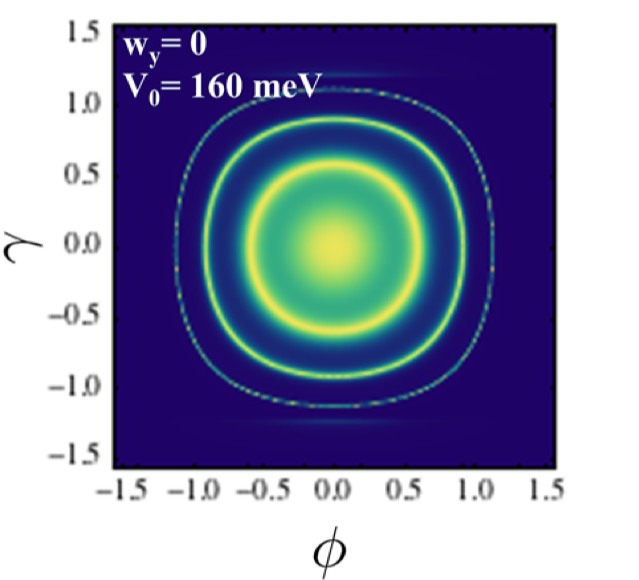
\includegraphics[width = \linewidth]{fig/Chap 2/anomalous1.png}
            \caption{}
            \label{2fig:anomalous1}
        \end{subfigure}
        \begin{subfigure}[b]{0.4\linewidth}
            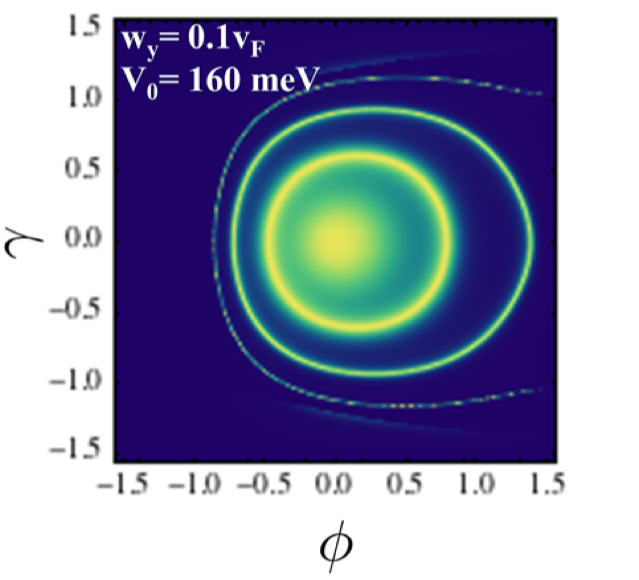
\includegraphics[width = \linewidth]{fig/Chap 2/anomalous2.png}
            \caption{}
            \label{2fig:anomalous2}
        \end{subfigure}

        \begin{subfigure}[b]{0.4\linewidth}
            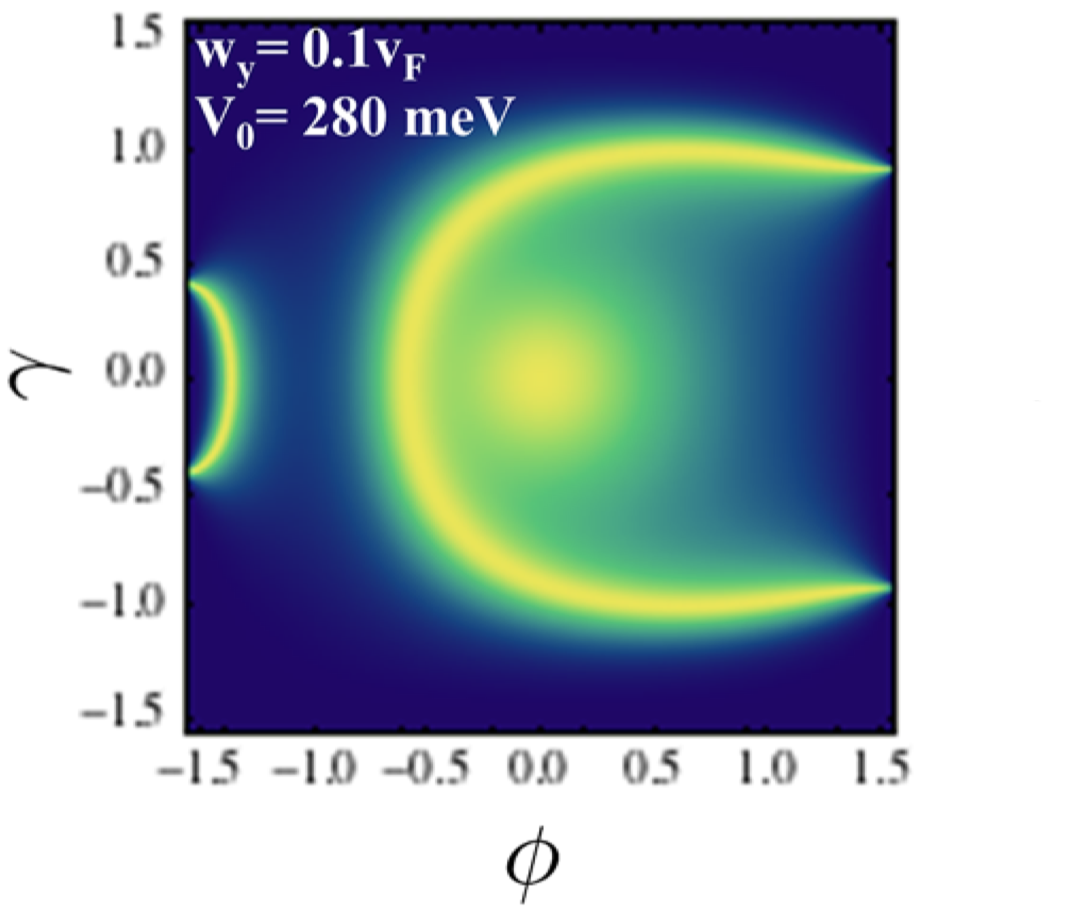
\includegraphics[width = \linewidth]{fig/Chap 2/anomalous3.png}
            \caption{}
            \label{2fig:anomalous3}
        \end{subfigure}
        \begin{subfigure}[b]{0.4\linewidth}
            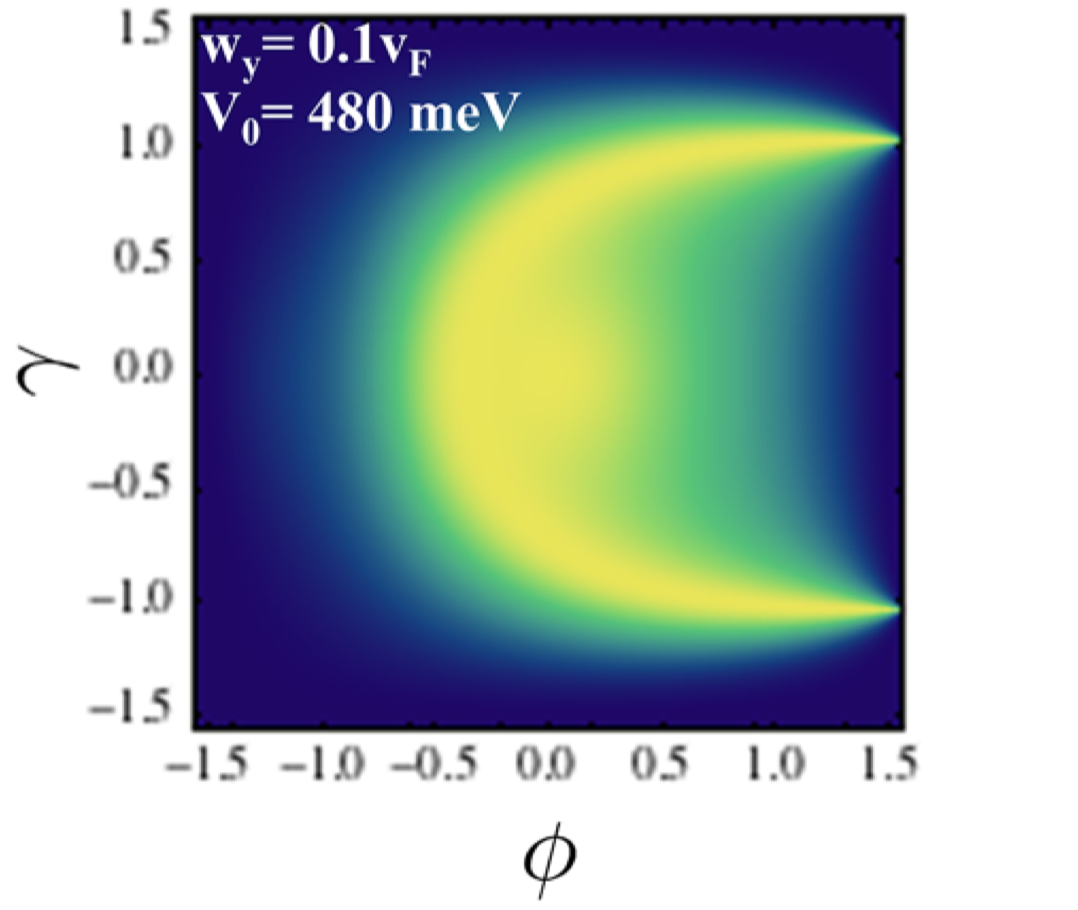
\includegraphics[width = \linewidth]{fig/Chap 2/anomalous4.png}
            \caption{}
            \label{2fig:anomalous4}
        \end{subfigure}

        \begin{subfigure}[b]{0.4\linewidth}
            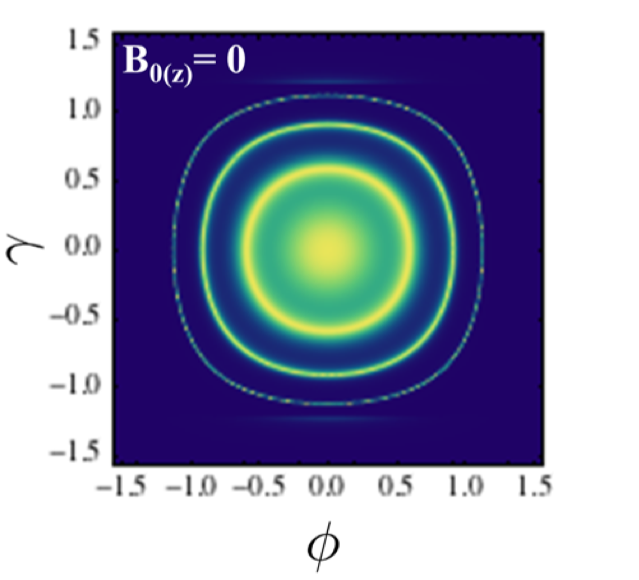
\includegraphics[width = \linewidth]{fig/Chap 2/anomalous5.png}
            \caption{}
            \label{2fig:anomalous5}
        \end{subfigure}
        \begin{subfigure}[b]{0.4\linewidth}
            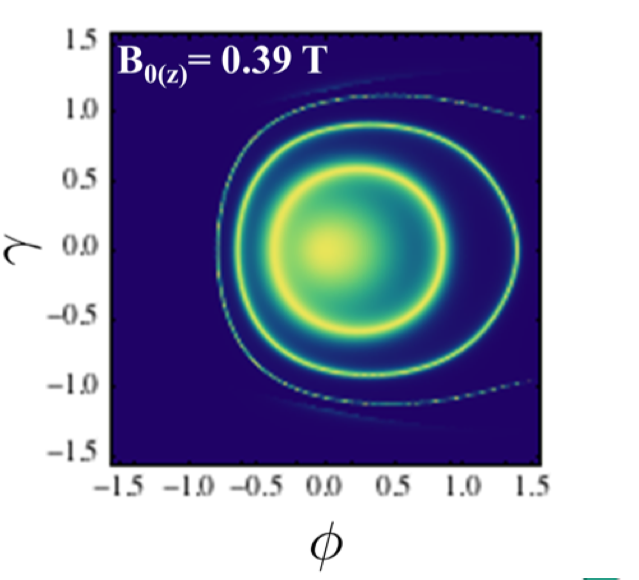
\includegraphics[width = \linewidth]{fig/Chap 2/anomalous6.png}
            \caption{}
            \label{2fig:anomalous6}
        \end{subfigure}
    \caption{anomalous tunneling}
    \label{2fig:anomalous}
    \end{figure}

    \begin{figure}[H]
        \centering
        \begin{subfigure}[b]{0.4\linewidth}
            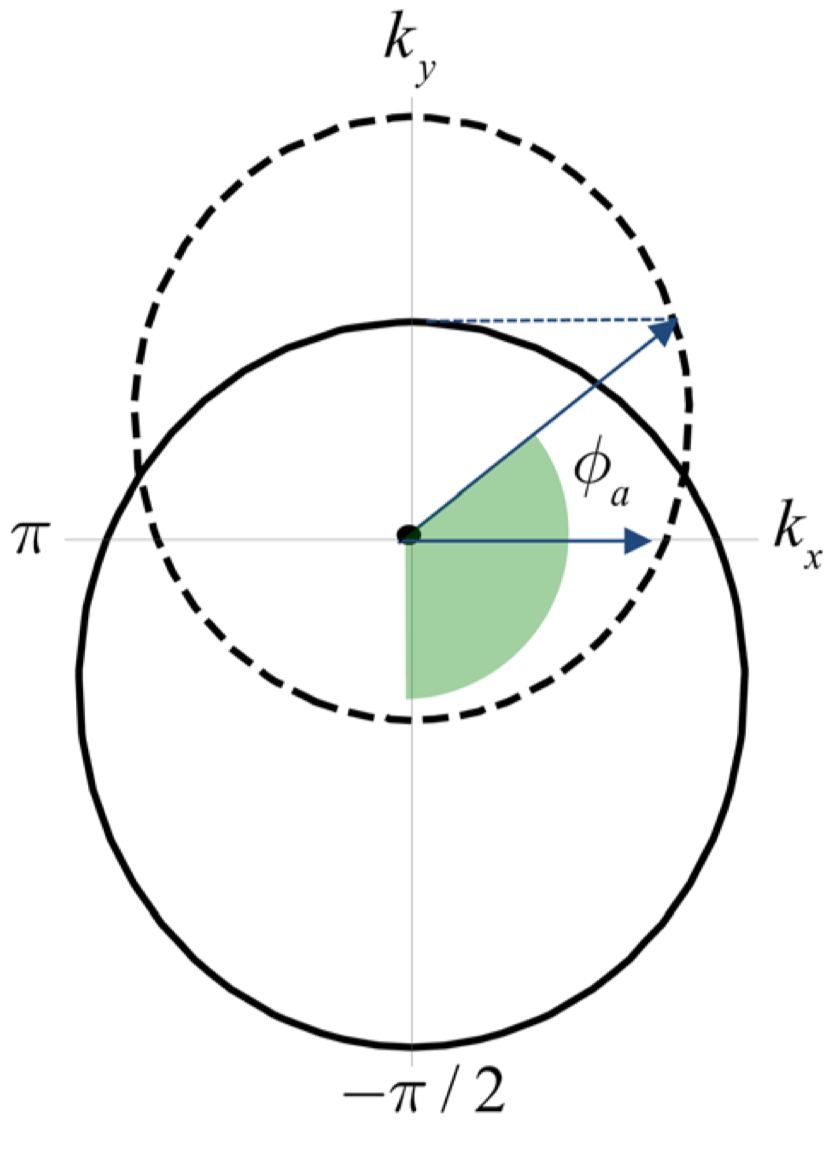
\includegraphics[width = \linewidth]{fig/Chap 2/anomalous fermi surface1.png}
            \caption{}
            \label{2fig:anomalous fermi surface1}
        \end{subfigure}
        \begin{subfigure}[b]{0.4\linewidth}
            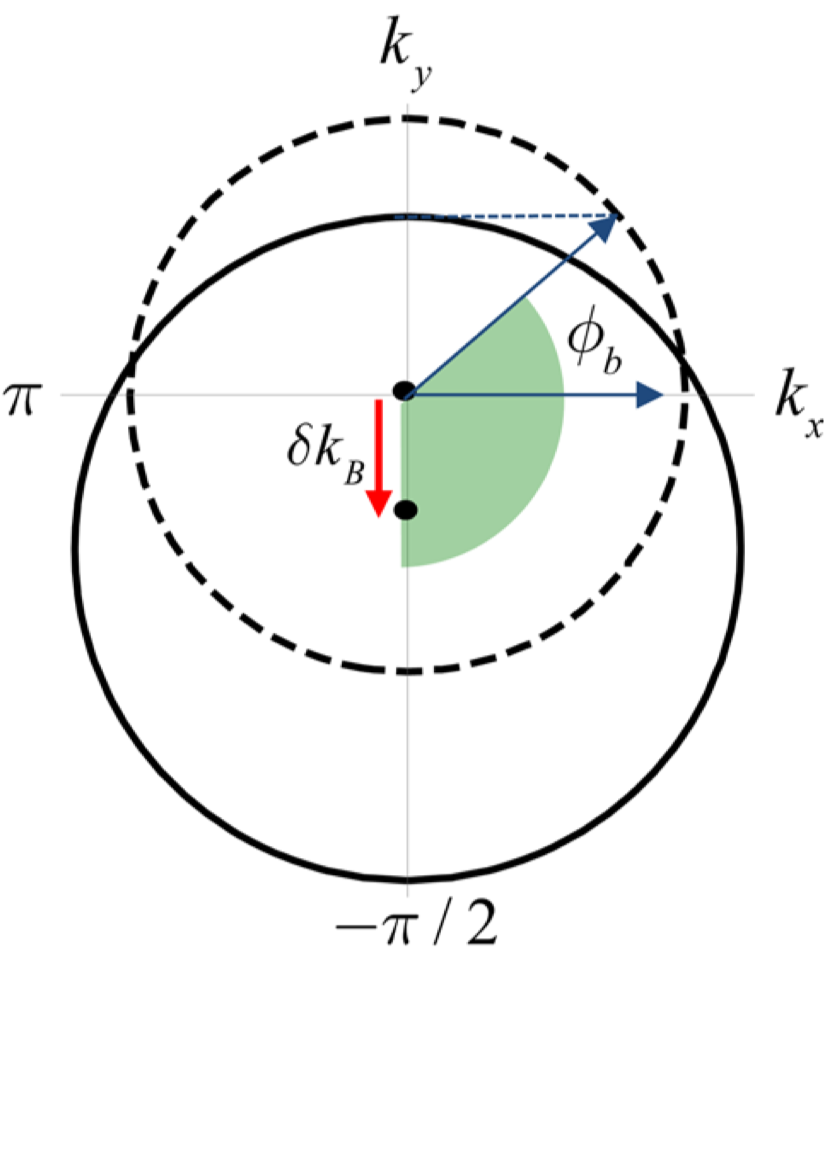
\includegraphics[width = \linewidth]{fig/Chap 2/anomalous fermi surface2.png}
            \caption{}
            \label{2fig:anomalous fermi surface2}
        \end{subfigure}
    \caption{anomalous Fermi surfaces}
    \label{2fig:anomalous fermi surface}
    \end{figure}